\documentclass[twoside]{article}

% Packages required by doxygen
\usepackage{fixltx2e}
\usepackage{calc}
\usepackage{doxygen}
\usepackage{graphicx}
\usepackage[utf8]{inputenc}
\usepackage{makeidx}
\usepackage{multicol}
\usepackage{multirow}
\PassOptionsToPackage{warn}{textcomp}
\usepackage{textcomp}
\usepackage[nointegrals]{wasysym}
\usepackage[table]{xcolor}

% Font selection
\usepackage[T1]{fontenc}
\usepackage{mathptmx}
\usepackage[scaled=.90]{helvet}
\usepackage{courier}
\usepackage{amssymb}
\usepackage{sectsty}
\renewcommand{\familydefault}{\sfdefault}
\allsectionsfont{%
  \fontseries{bc}\selectfont%
  \color{darkgray}%
}
\renewcommand{\DoxyLabelFont}{%
  \fontseries{bc}\selectfont%
  \color{darkgray}%
}
\newcommand{\+}{\discretionary{\mbox{\scriptsize$\hookleftarrow$}}{}{}}

% Page & text layout
\usepackage[screen]{geometry}
\tolerance=750
\hfuzz=15pt
\hbadness=750
\setlength{\emergencystretch}{15pt}
\setlength{\parindent}{0cm}
\setlength{\parskip}{0.2cm}
\makeatletter
\renewcommand{\paragraph}{%
  \@startsection{paragraph}{4}{0ex}{-1.0ex}{1.0ex}{%
    \normalfont\normalsize\bfseries\SS@parafont%
  }%
}
\renewcommand{\subparagraph}{%
  \@startsection{subparagraph}{5}{0ex}{-1.0ex}{1.0ex}{%
    \normalfont\normalsize\bfseries\SS@subparafont%
  }%
}
\makeatother

% Headers & footers
\usepackage{fancyhdr}
\pagestyle{fancyplain}
\fancyhead[LE]{\fancyplain{}{\bfseries\thepage}}
\fancyhead[CE]{\fancyplain{}{}}
\fancyhead[RE]{\fancyplain{}{\bfseries\leftmark}}
\fancyhead[LO]{\fancyplain{}{\bfseries\rightmark}}
\fancyhead[CO]{\fancyplain{}{}}
\fancyhead[RO]{\fancyplain{}{\bfseries\thepage}}
\fancyfoot[LE]{\fancyplain{}{}}
\fancyfoot[CE]{\fancyplain{}{}}
\fancyfoot[RE]{\fancyplain{}{\bfseries\scriptsize Generated on Sat Nov 4 2017 01\+:40\+:59 for Lab5 by Doxygen }}
\fancyfoot[LO]{\fancyplain{}{\bfseries\scriptsize Generated on Sat Nov 4 2017 01\+:40\+:59 for Lab5 by Doxygen }}
\fancyfoot[CO]{\fancyplain{}{}}
\fancyfoot[RO]{\fancyplain{}{}}
\renewcommand{\footrulewidth}{0.4pt}
\renewcommand{\sectionmark}[1]{%
  \markright{\thesection\ #1}%
}

% Indices & bibliography
\usepackage{natbib}
\usepackage[titles]{tocloft}
\setcounter{tocdepth}{3}
\setcounter{secnumdepth}{5}
\makeindex

% Packages requested by user
\usepackage{titlesec}

% Hyperlinks (required, but should be loaded last)
\usepackage{ifpdf}
\ifpdf
  \usepackage[pdftex,pagebackref=true]{hyperref}
\else
  \usepackage[ps2pdf,pagebackref=true]{hyperref}
\fi
\hypersetup{%
  colorlinks=true,%
  linkcolor=blue,%
  citecolor=blue,%
  unicode%
}

% Custom commands
\newcommand{\clearemptydoublepage}{%
  \newpage{\pagestyle{empty}\cleardoublepage}%
}


\newcommand{\sectionbreak}{\clearpage}

\begin{document}

% Titlepage & ToC
\hypersetup{pageanchor=false,
             bookmarks=true,
             bookmarksnumbered=true,
             pdfencoding=unicode
            }
\pagenumbering{roman}
\begin{titlepage}
\vspace*{7cm}
\begin{center}%
{\Large Lab5 }\\
\vspace*{1cm}
{\large Generated by Doxygen 1.8.8}\\
\vspace*{0.5cm}
{\small Sat Nov 4 2017 01:40:59}\\
\end{center}
\end{titlepage}
\tableofcontents
\pagenumbering{arabic}
\hypersetup{pageanchor=true}

%--- Begin generated contents ---
\section{read\+Data}
\label{readData}
\hypertarget{readData}{}
read some columns from file f snd store them in aqi array


\begin{DoxyParams}{Parameters}
{\em f} & filename \\
\hline
{\em aqi} & array to put data in \\
\hline
{\em n} & number of elements in the array \\
\hline
{\em read} & the first string in the file f and return it read the file and store the valuse into the array of structs we store the county names and the A\+Q\+I (airquality index of that county) \\
\hline
\end{DoxyParams}

\section{count\+Rows}
\label{countRows}
\hypertarget{countRows}{}
This program will count the rows in the .csv file. Everytime a new row is read n( the counter) gets incremented till the end 
\begin{DoxyParams}{Parameters}
{\em f} & The string that is the filename \\
\hline
{\em out} & we return n the number of rows \\
\hline
\end{DoxyParams}

\section{overloading}
\label{operator}
\hypertarget{operator}{}
This is the operator overloading pages I overloaded the $>$, $<$, $>$=, and $<$= operators This was done so I could compare the A\+Q\+I values specifically to one another without having to chang the authors code 
\section{addtimes}
\label{addtimes}
\hypertarget{addtimes}{}
This function reads the times it takes for the sorting algorithms to complete and then writes them into a file. that file is called times.\+txt


\begin{DoxyParams}{Parameters}
{\em filename} & the filename you want to it to write to \\
\hline
{\em inputstring} & the string you want to output \\
\hline
\end{DoxyParams}

\section{readtimes}
\label{readtimes}
\hypertarget{readtimes}{}
Void function to read the information in a file and dispaly it No parameters, Called in main. Select Time in html to see the exact output of this function 
\section{Specification}
\label{Specification}
\hypertarget{Specification}{}
This is the English-\/\+Italian Dictionary program. The user can input an English word and the program will provide translation of the word. The current file the program uses to translate is and English to Italian Dictionary If the word that user enters is not in the program the the user can add the word into the dictionary by following the instructions given by the program.

Freatures\+:

1) The instructures are clear and concise to understand.

2) The ability to add words into the dictionary/program for later use.

3) Operator overlaoding to improve effiecncy of program. 
\section{Analysis}
\label{Analysis}
\hypertarget{Analysis}{}
When the user goes to the html page the program is already running. Here the user will be greeted by 6 options to select from. 5 of these options are sorting algorithms the other one is an option to see the times it takes for them to sort. When a sort is selected the page will load the name of the sort and then all the sorted info below it. Th fastest sort was quick sort which took less than a second. The slowest was bubble which varied from 40 seconds to 3 minutes. 
\section{Design}
\label{Design}
\hypertarget{Design}{}
Html was what we used to create the U\+I for this lab. T\+He translation program however was done in C++. We implemented a binary tree which basically allows us to store elements that can reference elements lower than it. Like tree -\/$>$ branches -\/$>$ twigs -\/$>$ leaves. The idea is that only an element of lower value can be stored in bottom of another element and lower is on the left and greater on the right. So in our lab a . was considered lower and a -\/ was conidered higher. This allowed us to reference letters within the tree very quickly. 
\section{Test}
\label{Test}
\hypertarget{Test}{}
 


 
\section{Class Index}
\subsection{Class List}
Here are the classes, structs, unions and interfaces with brief descriptions\+:\begin{DoxyCompactList}
\item\contentsline{section}{\hyperlink{structFRAGMENT}{F\+R\+A\+G\+M\+E\+N\+T} }{\pageref{structFRAGMENT}}{}
\item\contentsline{section}{\hyperlink{structMUSICELMT}{M\+U\+S\+I\+C\+E\+L\+M\+T} }{\pageref{structMUSICELMT}}{}
\item\contentsline{section}{\hyperlink{structNOTE}{N\+O\+T\+E} }{\pageref{structNOTE}}{}
\item\contentsline{section}{\hyperlink{structSTACK}{S\+T\+A\+C\+K} }{\pageref{structSTACK}}{}
\end{DoxyCompactList}

\section{File Index}
\subsection{File List}
Here is a list of all files with brief descriptions\+:\begin{DoxyCompactList}
\item\contentsline{section}{\hyperlink{addWords_8cpp}{add\+Words.\+cpp} }{\pageref{addWords_8cpp}}{}
\item\contentsline{section}{\hyperlink{foundWord_8cpp}{found\+Word.\+cpp} }{\pageref{foundWord_8cpp}}{}
\item\contentsline{section}{\hyperlink{lab_8cpp}{lab.\+cpp} }{\pageref{lab_8cpp}}{}
\item\contentsline{section}{\hyperlink{lab_8h}{lab.\+h} }{\pageref{lab_8h}}{}
\item\contentsline{section}{\hyperlink{loadDictionary_8cpp}{load\+Dictionary.\+cpp} }{\pageref{loadDictionary_8cpp}}{}
\item\contentsline{section}{\hyperlink{main_8cpp}{main.\+cpp} }{\pageref{main_8cpp}}{}
\end{DoxyCompactList}

\section{Class Documentation}
\hypertarget{structAQIData}{\subsection{A\+Q\+I\+Data Struct Reference}
\label{structAQIData}\index{A\+Q\+I\+Data@{A\+Q\+I\+Data}}
}


{\ttfamily \#include $<$lab.\+h$>$}

\subsubsection*{Public Attributes}
\begin{DoxyCompactItemize}
\item 
string \hyperlink{structAQIData_a8491fd5d9608d9be9f820868780a97b8}{county}
\item 
int \hyperlink{structAQIData_a4078cc02f4de75228f0880ea84bdedc6}{A\+Q\+I}
\end{DoxyCompactItemize}


\subsubsection{Member Data Documentation}
\hypertarget{structAQIData_a4078cc02f4de75228f0880ea84bdedc6}{\index{A\+Q\+I\+Data@{A\+Q\+I\+Data}!A\+Q\+I@{A\+Q\+I}}
\index{A\+Q\+I@{A\+Q\+I}!A\+Q\+I\+Data@{A\+Q\+I\+Data}}
\paragraph[{A\+Q\+I}]{\setlength{\rightskip}{0pt plus 5cm}int A\+Q\+I\+Data\+::\+A\+Q\+I}}\label{structAQIData_a4078cc02f4de75228f0880ea84bdedc6}
\hypertarget{structAQIData_a8491fd5d9608d9be9f820868780a97b8}{\index{A\+Q\+I\+Data@{A\+Q\+I\+Data}!county@{county}}
\index{county@{county}!A\+Q\+I\+Data@{A\+Q\+I\+Data}}
\paragraph[{county}]{\setlength{\rightskip}{0pt plus 5cm}string A\+Q\+I\+Data\+::county}}\label{structAQIData_a8491fd5d9608d9be9f820868780a97b8}


The documentation for this struct was generated from the following file\+:\begin{DoxyCompactItemize}
\item 
\hyperlink{lab_8h}{lab.\+h}\end{DoxyCompactItemize}

\hypertarget{classMERGESORT}{\subsection{M\+E\+R\+G\+E\+S\+O\+R\+T$<$ A\+Q\+I\+Data $>$ Class Template Reference}
\label{classMERGESORT}\index{M\+E\+R\+G\+E\+S\+O\+R\+T$<$ A\+Q\+I\+Data $>$@{M\+E\+R\+G\+E\+S\+O\+R\+T$<$ A\+Q\+I\+Data $>$}}
}


{\ttfamily \#include $<$lab.\+h$>$}

\subsubsection*{Public Member Functions}
\begin{DoxyCompactItemize}
\item 
\hyperlink{classMERGESORT_a8965b6cdd1fedab95df230f65e094721}{M\+E\+R\+G\+E\+S\+O\+R\+T} (int n)
\item 
\hyperlink{classMERGESORT_a42c9dce7fc0c35538d0e948ba1c3be39}{$\sim$\+M\+E\+R\+G\+E\+S\+O\+R\+T} ()
\item 
void \hyperlink{classMERGESORT_ab3dba99ab686ac3a686c82fc41a91d61}{Sort} (\hyperlink{structAQIData}{A\+Q\+I\+Data} a\mbox{[}$\,$\mbox{]}, int n)
\end{DoxyCompactItemize}


\subsubsection{Constructor \& Destructor Documentation}
\hypertarget{classMERGESORT_a8965b6cdd1fedab95df230f65e094721}{\index{M\+E\+R\+G\+E\+S\+O\+R\+T@{M\+E\+R\+G\+E\+S\+O\+R\+T}!M\+E\+R\+G\+E\+S\+O\+R\+T@{M\+E\+R\+G\+E\+S\+O\+R\+T}}
\index{M\+E\+R\+G\+E\+S\+O\+R\+T@{M\+E\+R\+G\+E\+S\+O\+R\+T}!M\+E\+R\+G\+E\+S\+O\+R\+T@{M\+E\+R\+G\+E\+S\+O\+R\+T}}
\paragraph[{M\+E\+R\+G\+E\+S\+O\+R\+T}]{\setlength{\rightskip}{0pt plus 5cm}template$<$class A\+Q\+I\+Data$>$ {\bf M\+E\+R\+G\+E\+S\+O\+R\+T}$<$ {\bf A\+Q\+I\+Data} $>$\+::{\bf M\+E\+R\+G\+E\+S\+O\+R\+T} (
\begin{DoxyParamCaption}
\item[{int}]{n}
\end{DoxyParamCaption}
)\hspace{0.3cm}{\ttfamily [inline]}}}\label{classMERGESORT_a8965b6cdd1fedab95df230f65e094721}

\begin{DoxyCode}
51 \{work = \textcolor{keyword}{new} \hyperlink{structAQIData}{AQIData}[n]; \}
\end{DoxyCode}
\hypertarget{classMERGESORT_a42c9dce7fc0c35538d0e948ba1c3be39}{\index{M\+E\+R\+G\+E\+S\+O\+R\+T@{M\+E\+R\+G\+E\+S\+O\+R\+T}!````~M\+E\+R\+G\+E\+S\+O\+R\+T@{$\sim$\+M\+E\+R\+G\+E\+S\+O\+R\+T}}
\index{````~M\+E\+R\+G\+E\+S\+O\+R\+T@{$\sim$\+M\+E\+R\+G\+E\+S\+O\+R\+T}!M\+E\+R\+G\+E\+S\+O\+R\+T@{M\+E\+R\+G\+E\+S\+O\+R\+T}}
\paragraph[{$\sim$\+M\+E\+R\+G\+E\+S\+O\+R\+T}]{\setlength{\rightskip}{0pt plus 5cm}template$<$class A\+Q\+I\+Data$>$ {\bf M\+E\+R\+G\+E\+S\+O\+R\+T}$<$ {\bf A\+Q\+I\+Data} $>$\+::$\sim${\bf M\+E\+R\+G\+E\+S\+O\+R\+T} (
\begin{DoxyParamCaption}
{}
\end{DoxyParamCaption}
)\hspace{0.3cm}{\ttfamily [inline]}}}\label{classMERGESORT_a42c9dce7fc0c35538d0e948ba1c3be39}

\begin{DoxyCode}
53 \{\textcolor{keyword}{delete} [] work;\}
\end{DoxyCode}


\subsubsection{Member Function Documentation}
\hypertarget{classMERGESORT_ab3dba99ab686ac3a686c82fc41a91d61}{\index{M\+E\+R\+G\+E\+S\+O\+R\+T@{M\+E\+R\+G\+E\+S\+O\+R\+T}!Sort@{Sort}}
\index{Sort@{Sort}!M\+E\+R\+G\+E\+S\+O\+R\+T@{M\+E\+R\+G\+E\+S\+O\+R\+T}}
\paragraph[{Sort}]{\setlength{\rightskip}{0pt plus 5cm}template$<$class A\+Q\+I\+Data $>$ void {\bf M\+E\+R\+G\+E\+S\+O\+R\+T}$<$ {\bf A\+Q\+I\+Data} $>$\+::Sort (
\begin{DoxyParamCaption}
\item[{{\bf A\+Q\+I\+Data}}]{a\mbox{[}$\,$\mbox{]}, }
\item[{int}]{n}
\end{DoxyParamCaption}
)}}\label{classMERGESORT_ab3dba99ab686ac3a686c82fc41a91d61}

\begin{DoxyCode}
78 \{
79     \textcolor{keywordtype}{int} n1, n2;
80     \hyperlink{structAQIData}{AQIData} *a2;
81     \textcolor{keywordflow}{if} (n <= 2) \{ \textcolor{comment}{//Base Case }
82         \textcolor{keywordflow}{if} ( n== 2 && a[1] < a[0])
83             Swap(a[0], a[1]);
84         \}
85         \textcolor{keywordflow}{else} \{ \textcolor{comment}{// Recursive case:}
86             n1 = n/2; n2 = n - n1;
87             a2 = &a[n1];
88             
89             \hyperlink{classMERGESORT_ab3dba99ab686ac3a686c82fc41a91d61}{Sort}(a, n1);
90             \hyperlink{classMERGESORT_ab3dba99ab686ac3a686c82fc41a91d61}{Sort}(a2, n2);
91             Merge(a, n1, a2, n2);
92         \}
93 \}
\end{DoxyCode}


The documentation for this class was generated from the following files\+:\begin{DoxyCompactItemize}
\item 
\hyperlink{lab_8h}{lab.\+h}\item 
\hyperlink{SOMETYPE_8hpp}{S\+O\+M\+E\+T\+Y\+P\+E.\+hpp}\end{DoxyCompactItemize}

\hypertarget{classQUICKSORT}{\subsection{Q\+U\+I\+C\+K\+S\+O\+R\+T$<$ A\+Q\+I\+Data $>$ Class Template Reference}
\label{classQUICKSORT}\index{Q\+U\+I\+C\+K\+S\+O\+R\+T$<$ A\+Q\+I\+Data $>$@{Q\+U\+I\+C\+K\+S\+O\+R\+T$<$ A\+Q\+I\+Data $>$}}
}


{\ttfamily \#include $<$lab.\+h$>$}

\subsubsection*{Public Member Functions}
\begin{DoxyCompactItemize}
\item 
void \hyperlink{classQUICKSORT_a887986883eb752498aac3e329d993ce5}{Sort} (\hyperlink{structAQIData}{A\+Q\+I\+Data} a\mbox{[}$\,$\mbox{]}, int n)
\end{DoxyCompactItemize}


\subsubsection{Member Function Documentation}
\hypertarget{classQUICKSORT_a887986883eb752498aac3e329d993ce5}{\index{Q\+U\+I\+C\+K\+S\+O\+R\+T@{Q\+U\+I\+C\+K\+S\+O\+R\+T}!Sort@{Sort}}
\index{Sort@{Sort}!Q\+U\+I\+C\+K\+S\+O\+R\+T@{Q\+U\+I\+C\+K\+S\+O\+R\+T}}
\paragraph[{Sort}]{\setlength{\rightskip}{0pt plus 5cm}template$<$class A\+Q\+I\+Data $>$ void {\bf Q\+U\+I\+C\+K\+S\+O\+R\+T}$<$ {\bf A\+Q\+I\+Data} $>$\+::Sort (
\begin{DoxyParamCaption}
\item[{{\bf A\+Q\+I\+Data}}]{a\mbox{[}$\,$\mbox{]}, }
\item[{int}]{n}
\end{DoxyParamCaption}
)}}\label{classQUICKSORT_a887986883eb752498aac3e329d993ce5}

\begin{DoxyCode}
163 \{
164     \textcolor{keywordtype}{int} p;
165     
166     \textcolor{keywordflow}{if} (n <=2) \{
167         \textcolor{keywordflow}{if} (n ==2 && a[1] < a[0])
168             Swap(a[0], a[1]);
169         \}
170         \textcolor{keywordflow}{else} \{
171             p = Split(a, n);
172             \hyperlink{classQUICKSORT_a887986883eb752498aac3e329d993ce5}{Sort}(a, p);
173             \hyperlink{classQUICKSORT_a887986883eb752498aac3e329d993ce5}{Sort}(&a[p+1], n-p-1);
174         \}
175     \}
\end{DoxyCode}


The documentation for this class was generated from the following files\+:\begin{DoxyCompactItemize}
\item 
\hyperlink{lab_8h}{lab.\+h}\item 
\hyperlink{SOMETYPE_8hpp}{S\+O\+M\+E\+T\+Y\+P\+E.\+hpp}\end{DoxyCompactItemize}

\section{File Documentation}
\hypertarget{addtimes_8cpp}{\subsection{addtimes.\+cpp File Reference}
\label{addtimes_8cpp}\index{addtimes.\+cpp@{addtimes.\+cpp}}
}
{\ttfamily \#include \char`\"{}lab.\+h\char`\"{}}\\*
\subsubsection*{Functions}
\begin{DoxyCompactItemize}
\item 
bool \hyperlink{addtimes_8cpp_a7a7719446a70a6db5d33348671d0e8c5}{addtimes} (string filename, string inputstring)
\end{DoxyCompactItemize}


\subsubsection{Function Documentation}
\hypertarget{addtimes_8cpp_a7a7719446a70a6db5d33348671d0e8c5}{\index{addtimes.\+cpp@{addtimes.\+cpp}!addtimes@{addtimes}}
\index{addtimes@{addtimes}!addtimes.\+cpp@{addtimes.\+cpp}}
\paragraph[{addtimes}]{\setlength{\rightskip}{0pt plus 5cm}bool addtimes (
\begin{DoxyParamCaption}
\item[{string}]{filename, }
\item[{string}]{inputstring}
\end{DoxyParamCaption}
)}}\label{addtimes_8cpp_a7a7719446a70a6db5d33348671d0e8c5}

\begin{DoxyCode}
3 \{
4     
5     ofstream inpfile(filename, ios::app); 
6     inpfile << inputstring << endl;
7     inpfile.close();
8     \textcolor{keywordflow}{return} \textcolor{keyword}{true};
9 \}
\end{DoxyCode}

\hypertarget{countRows_8cpp}{\subsection{count\+Rows.\+cpp File Reference}
\label{countRows_8cpp}\index{count\+Rows.\+cpp@{count\+Rows.\+cpp}}
}
{\ttfamily \#include \char`\"{}lab.\+h\char`\"{}}\\*
\subsubsection*{Functions}
\begin{DoxyCompactItemize}
\item 
int \hyperlink{countRows_8cpp_af79b062a38e004faf58461580fe91f54}{count\+Rows} (string f)
\end{DoxyCompactItemize}


\subsubsection{Function Documentation}
\hypertarget{countRows_8cpp_af79b062a38e004faf58461580fe91f54}{\index{count\+Rows.\+cpp@{count\+Rows.\+cpp}!count\+Rows@{count\+Rows}}
\index{count\+Rows@{count\+Rows}!count\+Rows.\+cpp@{count\+Rows.\+cpp}}
\paragraph[{count\+Rows}]{\setlength{\rightskip}{0pt plus 5cm}int count\+Rows (
\begin{DoxyParamCaption}
\item[{string}]{f}
\end{DoxyParamCaption}
)}}\label{countRows_8cpp_af79b062a38e004faf58461580fe91f54}

\begin{DoxyCode}
3 \{
4     std::ifstream ifs(f.c\_str());
5     \textcolor{keywordtype}{int} n = 0;
6     \textcolor{keywordtype}{string} s;
7     \textcolor{keywordflow}{while}(getline(ifs,s)) n++;
8     
9     
10     \textcolor{keywordflow}{return} n;
11 \}
\end{DoxyCode}

\hypertarget{info_8cpp}{\subsection{info.\+cpp File Reference}
\label{info_8cpp}\index{info.\+cpp@{info.\+cpp}}
}
{\ttfamily \#include \char`\"{}lab.\+h\char`\"{}}\\*
\subsubsection*{Functions}
\begin{DoxyCompactItemize}
\item 
int \hyperlink{info_8cpp_a7d274093c26112507ac1ed67d7d1afc8}{average} ()
\end{DoxyCompactItemize}


\subsubsection{Function Documentation}
\hypertarget{info_8cpp_a7d274093c26112507ac1ed67d7d1afc8}{\index{info.\+cpp@{info.\+cpp}!average@{average}}
\index{average@{average}!info.\+cpp@{info.\+cpp}}
\paragraph[{average}]{\setlength{\rightskip}{0pt plus 5cm}int average (
\begin{DoxyParamCaption}
{}
\end{DoxyParamCaption}
)}}\label{info_8cpp_a7d274093c26112507ac1ed67d7d1afc8}

\begin{DoxyCode}
4 \{
5     
6     
7     
8 \}
\end{DoxyCode}

\hypertarget{lab_8h}{\subsection{lab.\+h File Reference}
\label{lab_8h}\index{lab.\+h@{lab.\+h}}
}
{\ttfamily \#include $<$fstream$>$}\\*
{\ttfamily \#include $<$iostream$>$}\\*
{\ttfamily \#include $<$string$>$}\\*
Include dependency graph for lab.\+h\+:\nopagebreak
\begin{figure}[H]
\begin{center}
\leavevmode
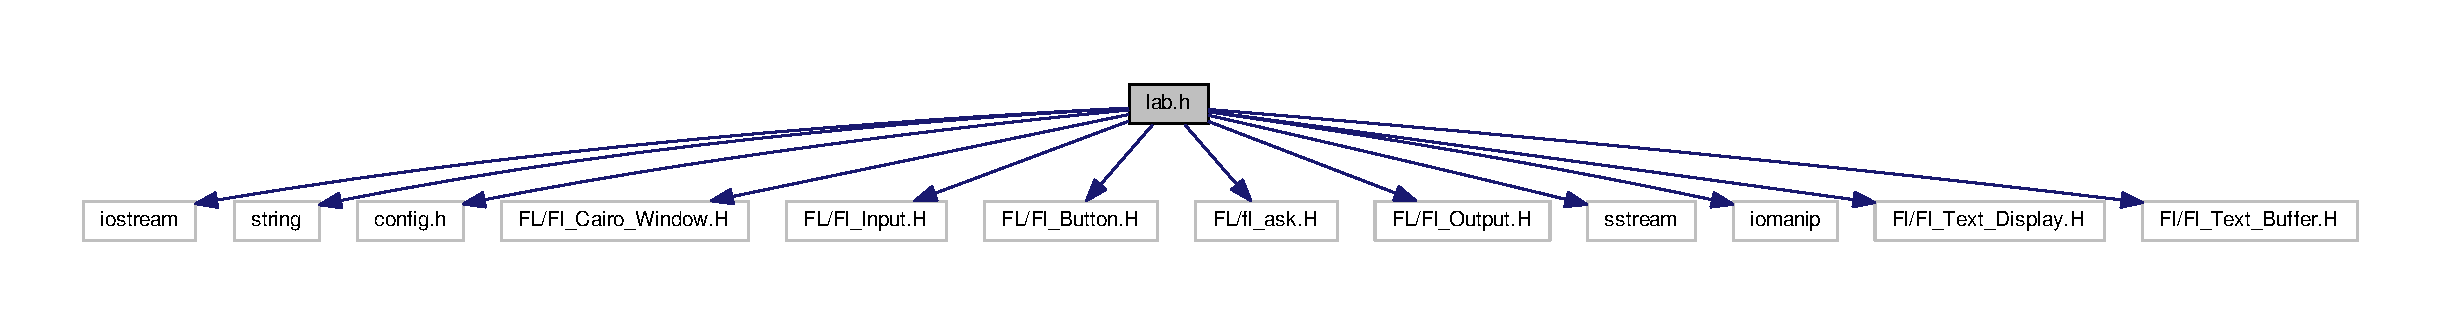
\includegraphics[width=261pt]{lab_8h__incl}
\end{center}
\end{figure}
This graph shows which files directly or indirectly include this file\+:\nopagebreak
\begin{figure}[H]
\begin{center}
\leavevmode
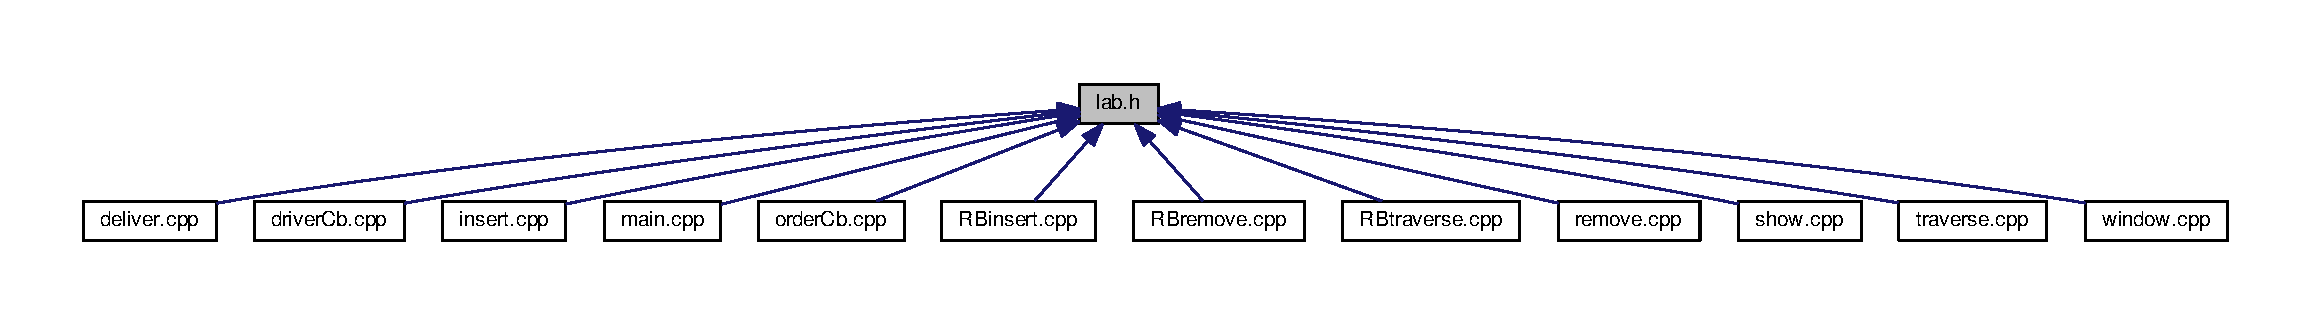
\includegraphics[width=350pt]{lab_8h__dep__incl}
\end{center}
\end{figure}
\subsubsection*{Classes}
\begin{DoxyCompactItemize}
\item 
struct \hyperlink{structNODE}{N\+O\+D\+E}
\begin{DoxyCompactList}\small\item\em City Structure. \end{DoxyCompactList}\end{DoxyCompactItemize}
\subsubsection*{Enumerations}
\begin{DoxyCompactItemize}
\item 
enum \hyperlink{lab_8h_a32c27cc471df37f4fc818d65de0a56c4}{S\+T\+A\+T\+U\+S} \{ \hyperlink{lab_8h_a32c27cc471df37f4fc818d65de0a56c4aecedb56d1405a60c6069f4a0139bdec5}{F\+A\+I\+L\+E\+D}, 
\hyperlink{lab_8h_a32c27cc471df37f4fc818d65de0a56c4a2bc49ec37d6a5715dd23e85f1ff5bb59}{O\+K}
 \}
\end{DoxyCompactItemize}
\subsubsection*{Functions}
\begin{DoxyCompactItemize}
\item 
\hyperlink{lab_8h_a32c27cc471df37f4fc818d65de0a56c4}{S\+T\+A\+T\+U\+S} \hyperlink{lab_8h_a578b73f866dc4391d05ca0219f892495}{insert} (\hyperlink{structNODE}{N\+O\+D\+E} $\ast$\&head, std\+::string city)
\begin{DoxyCompactList}\small\item\em Insert inserts a new node at the beginning of the list. \end{DoxyCompactList}\item 
\hyperlink{lab_8h_a32c27cc471df37f4fc818d65de0a56c4}{S\+T\+A\+T\+U\+S} \hyperlink{lab_8h_abf14767ea6c86eb593d6f87fe77267e7}{insertinorder} (\hyperlink{structNODE}{N\+O\+D\+E} $\ast$\&head, std\+::string city)
\item 
\hyperlink{lab_8h_a32c27cc471df37f4fc818d65de0a56c4}{S\+T\+A\+T\+U\+S} \hyperlink{lab_8h_a9eb7dfa9761b11c255d499765ea70b75}{builddirectly} (\hyperlink{structNODE}{N\+O\+D\+E} $\ast$\&head, string cities)
\item 
void \hyperlink{lab_8h_a67a34562a85e577c0921c5d65c22decc}{destroylist} (\hyperlink{structNODE}{N\+O\+D\+E} $\ast$head)
\item 
void \hyperlink{lab_8h_a6b2cb293574fc5dc8d7a4897cacea16f}{displaylist} (\hyperlink{structNODE}{N\+O\+D\+E} $\ast$head)
\item 
\hyperlink{structNODE}{N\+O\+D\+E} $\ast$ \hyperlink{lab_8h_afd6087490d82489b892a41298eba4e60}{loadlist} (std\+::string filename)
\end{DoxyCompactItemize}


\subsubsection{Enumeration Type Documentation}
\hypertarget{lab_8h_a32c27cc471df37f4fc818d65de0a56c4}{\index{lab.\+h@{lab.\+h}!S\+T\+A\+T\+U\+S@{S\+T\+A\+T\+U\+S}}
\index{S\+T\+A\+T\+U\+S@{S\+T\+A\+T\+U\+S}!lab.\+h@{lab.\+h}}
\paragraph[{S\+T\+A\+T\+U\+S}]{\setlength{\rightskip}{0pt plus 5cm}enum {\bf S\+T\+A\+T\+U\+S}}}\label{lab_8h_a32c27cc471df37f4fc818d65de0a56c4}
\begin{Desc}
\item[Enumerator]\par
\begin{description}
\index{F\+A\+I\+L\+E\+D@{F\+A\+I\+L\+E\+D}!lab.\+h@{lab.\+h}}\index{lab.\+h@{lab.\+h}!F\+A\+I\+L\+E\+D@{F\+A\+I\+L\+E\+D}}\item[{\em 
\hypertarget{lab_8h_a32c27cc471df37f4fc818d65de0a56c4aecedb56d1405a60c6069f4a0139bdec5}{F\+A\+I\+L\+E\+D}\label{lab_8h_a32c27cc471df37f4fc818d65de0a56c4aecedb56d1405a60c6069f4a0139bdec5}
}]\index{O\+K@{O\+K}!lab.\+h@{lab.\+h}}\index{lab.\+h@{lab.\+h}!O\+K@{O\+K}}\item[{\em 
\hypertarget{lab_8h_a32c27cc471df37f4fc818d65de0a56c4a2bc49ec37d6a5715dd23e85f1ff5bb59}{O\+K}\label{lab_8h_a32c27cc471df37f4fc818d65de0a56c4a2bc49ec37d6a5715dd23e85f1ff5bb59}
}]\end{description}
\end{Desc}

\begin{DoxyCode}
7 \{\hyperlink{lab_8h_a32c27cc471df37f4fc818d65de0a56c4aecedb56d1405a60c6069f4a0139bdec5}{FAILED}, \hyperlink{lab_8h_a32c27cc471df37f4fc818d65de0a56c4a2bc49ec37d6a5715dd23e85f1ff5bb59}{OK}\};
\end{DoxyCode}


\subsubsection{Function Documentation}
\hypertarget{lab_8h_a9eb7dfa9761b11c255d499765ea70b75}{\index{lab.\+h@{lab.\+h}!builddirectly@{builddirectly}}
\index{builddirectly@{builddirectly}!lab.\+h@{lab.\+h}}
\paragraph[{builddirectly}]{\setlength{\rightskip}{0pt plus 5cm}{\bf S\+T\+A\+T\+U\+S} builddirectly (
\begin{DoxyParamCaption}
\item[{{\bf N\+O\+D\+E} $\ast$\&}]{head, }
\item[{string}]{cities}
\end{DoxyParamCaption}
)}}\label{lab_8h_a9eb7dfa9761b11c255d499765ea70b75}

\begin{DoxyCode}
5 \{
6     \textcolor{keywordtype}{string} city;
7     \hyperlink{structNODE}{NODE}* tail; 
8     ifstream ifs(\textcolor{stringliteral}{"cities"});
9     \textcolor{keywordflow}{if} (! ifs) 
10     \textcolor{keywordflow}{return} \hyperlink{lab_8h_a32c27cc471df37f4fc818d65de0a56c4aecedb56d1405a60c6069f4a0139bdec5}{FAILED};
11     
12 \textcolor{keywordflow}{while}(ifs >> city) \{
13     \hyperlink{structNODE}{NODE} *newnode = \textcolor{keyword}{new} \hyperlink{structNODE}{NODE};
14     \textcolor{keywordflow}{if}(!newnode)
15     \textcolor{keywordflow}{return} \hyperlink{lab_8h_a32c27cc471df37f4fc818d65de0a56c4aecedb56d1405a60c6069f4a0139bdec5}{FAILED};
16     
17     newnode->\hyperlink{structNODE_a76c9a9603778b363e65bfe84da4bd72e}{city} = city;
18     
19     newnode->\hyperlink{structNODE_a078472e8ab2d2fe38e052f5c2a425618}{next} = 0;
20     
21      \textcolor{keywordflow}{if}(!tail) \{
22         head = newnode;\}
23     \textcolor{keywordflow}{else} \{
24         tail->\hyperlink{structNODE_a078472e8ab2d2fe38e052f5c2a425618}{next} = newnode;
25     \}
26     tail = newnode;
27     
28 \}
29 \}
\end{DoxyCode}
\hypertarget{lab_8h_a67a34562a85e577c0921c5d65c22decc}{\index{lab.\+h@{lab.\+h}!destroylist@{destroylist}}
\index{destroylist@{destroylist}!lab.\+h@{lab.\+h}}
\paragraph[{destroylist}]{\setlength{\rightskip}{0pt plus 5cm}void destroylist (
\begin{DoxyParamCaption}
\item[{{\bf N\+O\+D\+E} $\ast$}]{head}
\end{DoxyParamCaption}
)}}\label{lab_8h_a67a34562a85e577c0921c5d65c22decc}

\begin{DoxyParams}[1]{Parameters}
\mbox{\tt in}  & {\em head} & This is the only parameter the function takes.\\
\hline
\end{DoxyParams}
This function completely destroys the list.


\begin{DoxyImage}
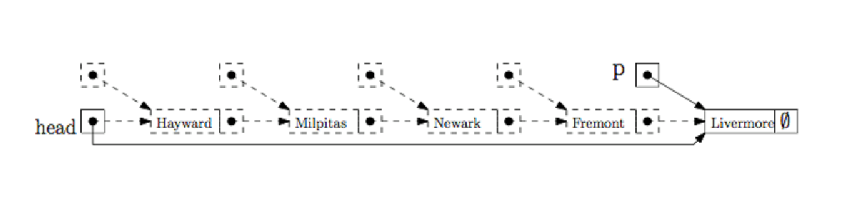
\includegraphics{destroylist1}
\caption{Linked List}
\end{DoxyImage}
 As you can see that this function points the head at the node and then deletes it severing the tie to the list 
\begin{DoxyCode}
14 \{
15     \hyperlink{structNODE}{NODE}* node;
16     \textcolor{keywordflow}{for}(node = head; node; node = node->\hyperlink{structNODE_a078472e8ab2d2fe38e052f5c2a425618}{next})
17     \{
18         cout << \textcolor{stringliteral}{"deleting: "}
19             << node->\hyperlink{structNODE_a76c9a9603778b363e65bfe84da4bd72e}{city} << std::endl;
20         \hyperlink{structNODE}{NODE}* tmp = head->\hyperlink{structNODE_a078472e8ab2d2fe38e052f5c2a425618}{next};
21         \textcolor{keyword}{delete} head;
22         head = tmp;
23         
24     \}
25     
26 \}
\end{DoxyCode}
\hypertarget{lab_8h_a6b2cb293574fc5dc8d7a4897cacea16f}{\index{lab.\+h@{lab.\+h}!displaylist@{displaylist}}
\index{displaylist@{displaylist}!lab.\+h@{lab.\+h}}
\paragraph[{displaylist}]{\setlength{\rightskip}{0pt plus 5cm}void displaylist (
\begin{DoxyParamCaption}
\item[{{\bf N\+O\+D\+E} $\ast$}]{head}
\end{DoxyParamCaption}
)}}\label{lab_8h_a6b2cb293574fc5dc8d7a4897cacea16f}

\begin{DoxyParams}[1]{Parameters}
\mbox{\tt in}  & {\em head} & This fucntion only takes a pointer as an argument.\\
\hline
\end{DoxyParams}
This function displays/traverses the list This is what a linked list looks like to a user It traverses the list without manipulating any pointers. See the comments for further deatils 
\begin{DoxyCode}
11 \{
12     \textcolor{comment}{//first we set the node pointer equal to the head pointer}
13     \textcolor{comment}{//Then while node exists this loop continues}
14     \textcolor{comment}{//Then we set the pointer equal to the next pointer }
15 
16     \textcolor{keywordflow}{for}(\hyperlink{structNODE}{NODE}* node = head; node; node = node->\hyperlink{structNODE_a078472e8ab2d2fe38e052f5c2a425618}{next})
17     \textcolor{comment}{//This displays the data within the node}
18     cout << node->city << endl;
19 \}
\end{DoxyCode}
\hypertarget{lab_8h_a578b73f866dc4391d05ca0219f892495}{\index{lab.\+h@{lab.\+h}!insert@{insert}}
\index{insert@{insert}!lab.\+h@{lab.\+h}}
\paragraph[{insert}]{\setlength{\rightskip}{0pt plus 5cm}{\bf S\+T\+A\+T\+U\+S} insert (
\begin{DoxyParamCaption}
\item[{{\bf N\+O\+D\+E} $\ast$\&}]{head, }
\item[{std\+::string}]{city}
\end{DoxyParamCaption}
)}}\label{lab_8h_a578b73f866dc4391d05ca0219f892495}


Insert inserts a new node at the beginning of the list. 


\begin{DoxyParams}[1]{Parameters}
\mbox{\tt in,out}  & {\em head} & The head of the linked list \\
\hline
\mbox{\tt in}  & {\em city} & The data in the node being inserted \\
\hline
\end{DoxyParams}
\begin{DoxyReturn}{Returns}
A S\+T\+A\+T\+U\+S indicating if Insert was successful of not
\end{DoxyReturn}

\begin{DoxyParams}[1]{Parameters}
\mbox{\tt in,out}  & {\em head} & The head of the linked list \\
\hline
\mbox{\tt in}  & {\em city} & The data in the node being inserted \\
\hline
\end{DoxyParams}
\begin{DoxyReturn}{Returns}
A S\+T\+A\+T\+U\+S indicating if Insert was successful of not 
\begin{DoxyImage}
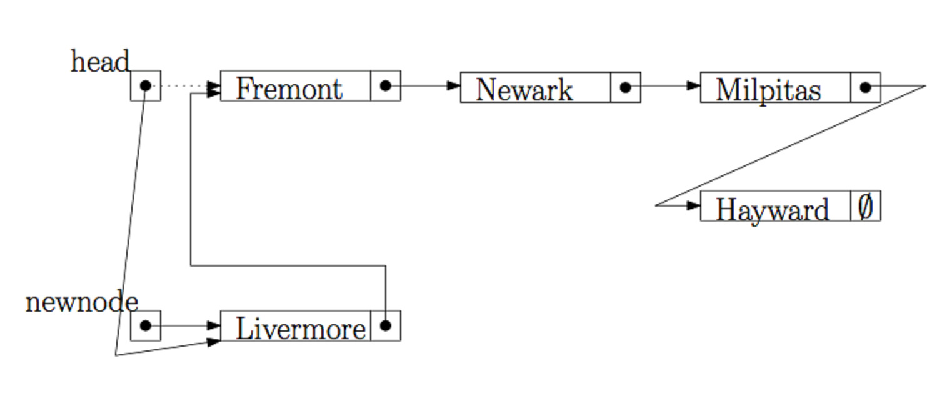
\includegraphics{insert}
\caption{Linked List}
\end{DoxyImage}
 
\end{DoxyReturn}

\begin{DoxyCode}
11 \{
12     \textcolor{comment}{//city = "Dublin"}
13     \hyperlink{structNODE}{NODE} *newnode;
14     
15     \textcolor{comment}{// Allocate a new node:}
16     
17     newnode = \textcolor{keyword}{new} \hyperlink{structNODE}{NODE};
18     \textcolor{keywordflow}{if} (!newnode)
19         \textcolor{keywordflow}{return} \hyperlink{lab_8h_a32c27cc471df37f4fc818d65de0a56c4aecedb56d1405a60c6069f4a0139bdec5}{FAILED}; 
20     \textcolor{comment}{//copy the info into the new node:}
21     
22     newnode->\hyperlink{structNODE_a76c9a9603778b363e65bfe84da4bd72e}{city} = city;
23     
24     \textcolor{comment}{//Link the new node to the list:}
25     
26     newnode->\hyperlink{structNODE_a078472e8ab2d2fe38e052f5c2a425618}{next} = head;
27     head = newnode; 
28     
29     \textcolor{keywordflow}{return} \hyperlink{lab_8h_a32c27cc471df37f4fc818d65de0a56c4a2bc49ec37d6a5715dd23e85f1ff5bb59}{OK}; 
30 \}
\end{DoxyCode}
\hypertarget{lab_8h_abf14767ea6c86eb593d6f87fe77267e7}{\index{lab.\+h@{lab.\+h}!insertinorder@{insertinorder}}
\index{insertinorder@{insertinorder}!lab.\+h@{lab.\+h}}
\paragraph[{insertinorder}]{\setlength{\rightskip}{0pt plus 5cm}{\bf S\+T\+A\+T\+U\+S} insertinorder (
\begin{DoxyParamCaption}
\item[{{\bf N\+O\+D\+E} $\ast$\&}]{head, }
\item[{std\+::string}]{city}
\end{DoxyParamCaption}
)}}\label{lab_8h_abf14767ea6c86eb593d6f87fe77267e7}

\begin{DoxyParams}[1]{Parameters}
\mbox{\tt in}  & {\em head,string} & This functions takes in the head and a string which is whatever city the user defines\\
\hline
\end{DoxyParams}
This function inserts a city into the list in a specific order.


\begin{DoxyImage}
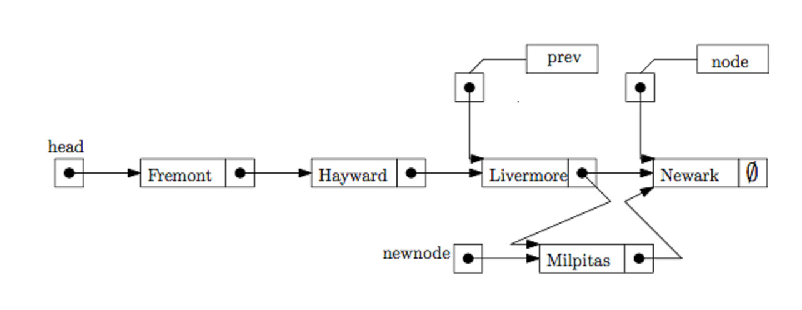
\includegraphics{insertinorder}
\caption{Linked List}
\end{DoxyImage}
 This shows how the pointers previous and next work as they traverse the list looking for a place to insert. Once it does it changes the pointers to add the value into the list 
\begin{DoxyCode}
16 \{
17     \hyperlink{structNODE}{NODE} *newnode;
18      \textcolor{comment}{// Allocate a new node:}
19      
20     newnode = \textcolor{keyword}{new} \hyperlink{structNODE}{NODE};
21     \textcolor{keywordflow}{if} (!newnode)
22         \textcolor{keywordflow}{return} \hyperlink{lab_8h_a32c27cc471df37f4fc818d65de0a56c4aecedb56d1405a60c6069f4a0139bdec5}{FAILED};
23         
24     \textcolor{comment}{// Copy the info into newnode:}
25     
26     newnode->\hyperlink{structNODE_a76c9a9603778b363e65bfe84da4bd72e}{city} = city;
27     
28     \textcolor{comment}{// LINK newnode to the list:}
29     \textcolor{comment}{// a) Find the right place to insert newnode (between "prev" and "node":}
30     
31     \hyperlink{structNODE}{NODE} *\hyperlink{structNODE}{NODE} = head, *prev = 0;
32     \textcolor{keywordflow}{while} (NODE && NODE->\hyperlink{structNODE_a76c9a9603778b363e65bfe84da4bd72e}{city} <= city) \{
33         \textcolor{comment}{//node->city <= city}
34     prev = NODE;        \textcolor{comment}{//advance node and prev}
35     NODE = NODE->\hyperlink{structNODE_a078472e8ab2d2fe38e052f5c2a425618}{next};
36 \}
37     \textcolor{comment}{// b) Link newnode between prev and node}
38     
39     newnode->\hyperlink{structNODE_a078472e8ab2d2fe38e052f5c2a425618}{next} = NODE; \textcolor{comment}{//append node to newnode}
40     \textcolor{keywordflow}{if} (prev)
41         prev->\hyperlink{structNODE_a078472e8ab2d2fe38e052f5c2a425618}{next} = newnode; \textcolor{comment}{//Insert after "prev"}
42     \textcolor{keywordflow}{else} 
43         head = newnode; \textcolor{comment}{//No prev: make new node the new head}
44         
45         \textcolor{keywordflow}{return} \hyperlink{lab_8h_a32c27cc471df37f4fc818d65de0a56c4a2bc49ec37d6a5715dd23e85f1ff5bb59}{OK};
46     \}
\end{DoxyCode}
\hypertarget{lab_8h_afd6087490d82489b892a41298eba4e60}{\index{lab.\+h@{lab.\+h}!loadlist@{loadlist}}
\index{loadlist@{loadlist}!lab.\+h@{lab.\+h}}
\paragraph[{loadlist}]{\setlength{\rightskip}{0pt plus 5cm}{\bf N\+O\+D\+E}$\ast$ loadlist (
\begin{DoxyParamCaption}
\item[{std\+::string}]{filename}
\end{DoxyParamCaption}
)}}\label{lab_8h_afd6087490d82489b892a41298eba4e60}
This function loads the dictionary into a linked list it takes the filename \char`\"{}cities\char`\"{} and loads that as cities the variable Then it uses the insert function to create the list after the head pointer. Then at the end it returns head so that we can use it in other functions. 
\begin{DoxyCode}
10 \{
11     \hyperlink{structNODE}{NODE}* head = 0; \textcolor{comment}{// this is where we declare the head as null to create the list}
12     std::ifstream ifs(filename.c\_str());
13     \textcolor{keywordtype}{string} city;
14     \textcolor{keywordflow}{while}(ifs >> city) 
15         \textcolor{keywordflow}{if}(\hyperlink{insert_8cpp_a578b73f866dc4391d05ca0219f892495}{insert}(head,city) == \hyperlink{lab_8h_a32c27cc471df37f4fc818d65de0a56c4aecedb56d1405a60c6069f4a0139bdec5}{FAILED})
16          cerr << \textcolor{stringliteral}{"error on insert\(\backslash\)n"};
17          
18     \textcolor{keywordflow}{return} head;
19 \}
\end{DoxyCode}

\hypertarget{main_8cpp}{\subsection{main.\+cpp File Reference}
\label{main_8cpp}\index{main.\+cpp@{main.\+cpp}}
}
{\ttfamily \#include \char`\"{}lab.\+h\char`\"{}}\\*
Include dependency graph for main.\+cpp\+:\nopagebreak
\begin{figure}[H]
\begin{center}
\leavevmode
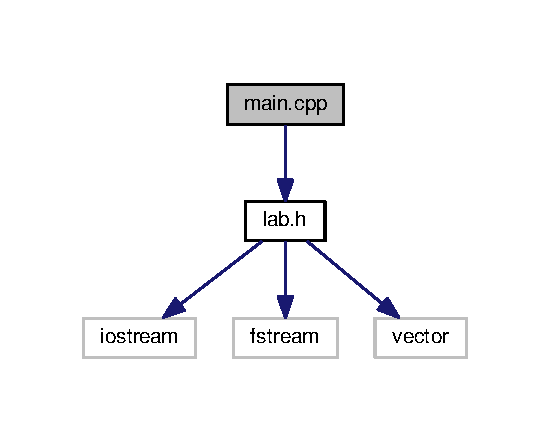
\includegraphics[width=264pt]{main_8cpp__incl}
\end{center}
\end{figure}
\subsubsection*{Functions}
\begin{DoxyCompactItemize}
\item 
int \hyperlink{main_8cpp_ae66f6b31b5ad750f1fe042a706a4e3d4}{main} ()
\end{DoxyCompactItemize}


\subsubsection{Function Documentation}
\hypertarget{main_8cpp_ae66f6b31b5ad750f1fe042a706a4e3d4}{\index{main.\+cpp@{main.\+cpp}!main@{main}}
\index{main@{main}!main.\+cpp@{main.\+cpp}}
\paragraph[{main}]{\setlength{\rightskip}{0pt plus 5cm}int main (
\begin{DoxyParamCaption}
{}
\end{DoxyParamCaption}
)}}\label{main_8cpp_ae66f6b31b5ad750f1fe042a706a4e3d4}
This is main function of the project. Contains the three fucntions (loaddictionary, foundwords, addwords) See comments for better understanding 
\begin{DoxyCode}
11 \{
12     vector<Entry> dict;
13     \textcolor{keywordtype}{string} word; \textcolor{comment}{// user inputs word}
14     \textcolor{keywordtype}{string} translation; \textcolor{comment}{// outputs translation}
15     \textcolor{keywordtype}{bool} ok, quit;
16     
17     ok = \hyperlink{lab_8h_ac18625e34f66c3bc052e07dfb0d3d219}{loaddictionary}(\textcolor{stringliteral}{"dict.dat"}, dict);
18     \textcolor{keywordflow}{if} (!ok) \{
19         cout << \textcolor{stringliteral}{" **** Cannot load Dictionary ***** \(\backslash\)n"};
20         \textcolor{keywordflow}{return} 1; \textcolor{comment}{//ERROR}
21     \}
22     
23     
24     \textcolor{keywordtype}{string} line;
25     
26  ifstream inpfile(\textcolor{stringliteral}{"dict.dat"}); \textcolor{comment}{//opening file again so that once updated }
27     \textcolor{keywordflow}{if} (!inpfile) \textcolor{keywordflow}{return} \textcolor{keyword}{false}; \textcolor{comment}{//the new information can be called without restarting the program}
28     
29     getline(inpfile, line);
30     cout << line << endl;
31     cout << \textcolor{stringliteral}{"Program by Samuel Jothimuthu"} <<endl;
32 
33     quit = \textcolor{keyword}{false};
34     \textcolor{keywordflow}{while} (!quit) \{ \textcolor{comment}{//iteration control structure}
35         \hyperlink{lab_8h_ac18625e34f66c3bc052e07dfb0d3d219}{loaddictionary}(\textcolor{stringliteral}{"dict.dat"}, dict);
36 
37         \textcolor{keywordtype}{string} choice; \textcolor{comment}{//simple choice of yes or no }
38         \textcolor{keywordtype}{string} newtran; \textcolor{comment}{//new translation for word user enters}
39         \textcolor{keywordtype}{string} inputstring; \textcolor{comment}{// the full string that will be appened to the file "dict.dat"}
40         cout << \textcolor{stringliteral}{"Enter a word or 'q' to quit ==> "};
41         cin >> word;
42         cin.ignore(80, \textcolor{charliteral}{'\(\backslash\)n'}); \textcolor{comment}{//this allows the console argument to execute but skipping the line}
43         \textcolor{keywordflow}{if} (word == \textcolor{stringliteral}{"q"}) 
44             quit = \textcolor{keyword}{true};
45         \textcolor{keywordflow}{else} \textcolor{keywordflow}{if} (\hyperlink{foundWord_8cpp_ae41eba27837d0aeea84fb5c6824388db}{foundword}( dict, word, translation)) \textcolor{comment}{//function must return true}
46             cout << translation << \textcolor{stringliteral}{"\(\backslash\)n\(\backslash\)n"};
47         \textcolor{keywordflow}{else} \textcolor{comment}{//The selection control structure}
48            \{ cout << word << \textcolor{stringliteral}{" --not in the dictionary. \(\backslash\)n Would you like to add it? (y/n)\(\backslash\)n"};
49             cin >> choice;
50             \textcolor{keywordflow}{if} (choice == \textcolor{stringliteral}{"y"}) \{ \textcolor{comment}{//any other input does not work. }
51                 cout << \textcolor{stringliteral}{"What is the Italian translation for "} << word << \textcolor{stringliteral}{"?"} << endl;
52                 cin >> newtran;
53                 inputstring = word + \textcolor{stringliteral}{"\(\backslash\)t"} + newtran; \textcolor{comment}{// this builds the full string that the program can
       then call upon.}
54                 \hyperlink{addWords_8cpp_ab5aa985d3bd8d2b89a2d5f35f38fb868}{addwords}(\textcolor{stringliteral}{"dict.dat"}, inputstring); \textcolor{comment}{//runs the addwords function, adding it into the
       file.}
55                 \}
56         \}
57         \}
58         \textcolor{keywordflow}{return} 0;
59     \}
\end{DoxyCode}

\hypertarget{overloading_8cpp}{\subsection{overloading.\+cpp File Reference}
\label{overloading_8cpp}\index{overloading.\+cpp@{overloading.\+cpp}}
}
{\ttfamily \#include \char`\"{}lab.\+h\char`\"{}}\\*
\subsubsection*{Functions}
\begin{DoxyCompactItemize}
\item 
bool \hyperlink{overloading_8cpp_a85332d2da1084afe152086facbe509a6}{operator$>$=} (const \hyperlink{structAQIData}{A\+Q\+I\+Data} \&lhs, const \hyperlink{structAQIData}{A\+Q\+I\+Data} \&rhs)
\item 
bool \hyperlink{overloading_8cpp_a8cd3ea0aed06a782e5dcf73049c0d4bd}{operator$<$=} (const \hyperlink{structAQIData}{A\+Q\+I\+Data} \&lhs, const \hyperlink{structAQIData}{A\+Q\+I\+Data} \&rhs)
\item 
bool \hyperlink{overloading_8cpp_a8458af03a840c0d3676203c4b02d3bfb}{operator$>$} (const \hyperlink{structAQIData}{A\+Q\+I\+Data} \&lhs, const \hyperlink{structAQIData}{A\+Q\+I\+Data} \&rhs)
\item 
bool \hyperlink{overloading_8cpp_a857de641d401861627c04f6af22db8f9}{operator$<$} (const \hyperlink{structAQIData}{A\+Q\+I\+Data} \&lhs, const \hyperlink{structAQIData}{A\+Q\+I\+Data} \&rhs)
\end{DoxyCompactItemize}


\subsubsection{Function Documentation}
\hypertarget{overloading_8cpp_a857de641d401861627c04f6af22db8f9}{\index{overloading.\+cpp@{overloading.\+cpp}!operator$<$@{operator$<$}}
\index{operator$<$@{operator$<$}!overloading.\+cpp@{overloading.\+cpp}}
\paragraph[{operator$<$}]{\setlength{\rightskip}{0pt plus 5cm}bool operator$<$ (
\begin{DoxyParamCaption}
\item[{const {\bf A\+Q\+I\+Data} \&}]{lhs, }
\item[{const {\bf A\+Q\+I\+Data} \&}]{rhs}
\end{DoxyParamCaption}
)}}\label{overloading_8cpp_a857de641d401861627c04f6af22db8f9}

\begin{DoxyCode}
24 \{
25     \textcolor{keywordflow}{return}(lhs.\hyperlink{structAQIData_a4078cc02f4de75228f0880ea84bdedc6}{AQI} < rhs.\hyperlink{structAQIData_a4078cc02f4de75228f0880ea84bdedc6}{AQI});
26 \}
\end{DoxyCode}
\hypertarget{overloading_8cpp_a8cd3ea0aed06a782e5dcf73049c0d4bd}{\index{overloading.\+cpp@{overloading.\+cpp}!operator$<$=@{operator$<$=}}
\index{operator$<$=@{operator$<$=}!overloading.\+cpp@{overloading.\+cpp}}
\paragraph[{operator$<$=}]{\setlength{\rightskip}{0pt plus 5cm}bool operator$<$= (
\begin{DoxyParamCaption}
\item[{const {\bf A\+Q\+I\+Data} \&}]{lhs, }
\item[{const {\bf A\+Q\+I\+Data} \&}]{rhs}
\end{DoxyParamCaption}
)}}\label{overloading_8cpp_a8cd3ea0aed06a782e5dcf73049c0d4bd}

\begin{DoxyCode}
14 \{
15     \textcolor{keywordflow}{return}(lhs.\hyperlink{structAQIData_a4078cc02f4de75228f0880ea84bdedc6}{AQI} <= rhs.\hyperlink{structAQIData_a4078cc02f4de75228f0880ea84bdedc6}{AQI});
16 \}
\end{DoxyCode}
\hypertarget{overloading_8cpp_a8458af03a840c0d3676203c4b02d3bfb}{\index{overloading.\+cpp@{overloading.\+cpp}!operator$>$@{operator$>$}}
\index{operator$>$@{operator$>$}!overloading.\+cpp@{overloading.\+cpp}}
\paragraph[{operator$>$}]{\setlength{\rightskip}{0pt plus 5cm}bool operator$>$ (
\begin{DoxyParamCaption}
\item[{const {\bf A\+Q\+I\+Data} \&}]{lhs, }
\item[{const {\bf A\+Q\+I\+Data} \&}]{rhs}
\end{DoxyParamCaption}
)}}\label{overloading_8cpp_a8458af03a840c0d3676203c4b02d3bfb}

\begin{DoxyCode}
19 \{
20     \textcolor{keywordflow}{return}(lhs.\hyperlink{structAQIData_a4078cc02f4de75228f0880ea84bdedc6}{AQI} > rhs.\hyperlink{structAQIData_a4078cc02f4de75228f0880ea84bdedc6}{AQI});
21 \}
\end{DoxyCode}
\hypertarget{overloading_8cpp_a85332d2da1084afe152086facbe509a6}{\index{overloading.\+cpp@{overloading.\+cpp}!operator$>$=@{operator$>$=}}
\index{operator$>$=@{operator$>$=}!overloading.\+cpp@{overloading.\+cpp}}
\paragraph[{operator$>$=}]{\setlength{\rightskip}{0pt plus 5cm}bool operator$>$= (
\begin{DoxyParamCaption}
\item[{const {\bf A\+Q\+I\+Data} \&}]{lhs, }
\item[{const {\bf A\+Q\+I\+Data} \&}]{rhs}
\end{DoxyParamCaption}
)}}\label{overloading_8cpp_a85332d2da1084afe152086facbe509a6}
This is the operator overloading pages I overloaded the $>$, $<$, $>$=, and $<$= operators This was done so I could compare the A\+Q\+I values specifically to one another without having to chang the authors code 
\begin{DoxyCode}
9 \{
10     \textcolor{keywordflow}{return}(lhs.\hyperlink{structAQIData_a4078cc02f4de75228f0880ea84bdedc6}{AQI} >= rhs.\hyperlink{structAQIData_a4078cc02f4de75228f0880ea84bdedc6}{AQI});
11 \}
\end{DoxyCode}

\hypertarget{readData_8cpp}{\subsection{read\+Data.\+cpp File Reference}
\label{readData_8cpp}\index{read\+Data.\+cpp@{read\+Data.\+cpp}}
}
{\ttfamily \#include \char`\"{}lab.\+h\char`\"{}}\\*
\subsubsection*{Functions}
\begin{DoxyCompactItemize}
\item 
void \hyperlink{readData_8cpp_afa2b122c9605683c5ad06505f8d3ea0a}{read\+Data} (string f, \hyperlink{structAQIData}{A\+Q\+I\+Data} aqi\mbox{[}$\,$\mbox{]}, int n)
\end{DoxyCompactItemize}


\subsubsection{Function Documentation}
\hypertarget{readData_8cpp_afa2b122c9605683c5ad06505f8d3ea0a}{\index{read\+Data.\+cpp@{read\+Data.\+cpp}!read\+Data@{read\+Data}}
\index{read\+Data@{read\+Data}!read\+Data.\+cpp@{read\+Data.\+cpp}}
\paragraph[{read\+Data}]{\setlength{\rightskip}{0pt plus 5cm}void read\+Data (
\begin{DoxyParamCaption}
\item[{string}]{f, }
\item[{{\bf A\+Q\+I\+Data}}]{aqi\mbox{[}$\,$\mbox{]}, }
\item[{int}]{n}
\end{DoxyParamCaption}
)}}\label{readData_8cpp_afa2b122c9605683c5ad06505f8d3ea0a}

\begin{DoxyCode}
10 \{
11     ifstream ifs (f.c\_str());
12     \textcolor{keywordtype}{string} s; \textcolor{keywordtype}{char} comma = \textcolor{charliteral}{','};
13     getline(ifs,s);
14     \textcolor{keywordflow}{for}( \textcolor{keywordtype}{int} i = 0; i < n ; i++) \{
15     getline(ifs,s,\textcolor{charliteral}{','}); \textcolor{comment}{//read and ignore the state}
16     getline(ifs, aqi[i].county, \textcolor{charliteral}{','});
17     getline(ifs,s,\textcolor{charliteral}{','});
18     getline(ifs,s,\textcolor{charliteral}{','}); \textcolor{comment}{//read and ignore state}
19     getline (ifs,s,\textcolor{charliteral}{','}); \textcolor{comment}{//read amd ind ignore the Days of AQI}
20     ifs >>  aqi[i].\hyperlink{structAQIData_a4078cc02f4de75228f0880ea84bdedc6}{AQI} >> comma;
21     getline(ifs,s);
22 \}
23     ifs.close();
24 \}
\end{DoxyCode}

\hypertarget{readtimes_8cpp}{\subsection{readtimes.\+cpp File Reference}
\label{readtimes_8cpp}\index{readtimes.\+cpp@{readtimes.\+cpp}}
}
{\ttfamily \#include \char`\"{}lab.\+h\char`\"{}}\\*
\subsubsection*{Functions}
\begin{DoxyCompactItemize}
\item 
void \hyperlink{readtimes_8cpp_abed4d504ddb0a41eff492be7984941f2}{readtimes} ()
\end{DoxyCompactItemize}


\subsubsection{Function Documentation}
\hypertarget{readtimes_8cpp_abed4d504ddb0a41eff492be7984941f2}{\index{readtimes.\+cpp@{readtimes.\+cpp}!readtimes@{readtimes}}
\index{readtimes@{readtimes}!readtimes.\+cpp@{readtimes.\+cpp}}
\paragraph[{readtimes}]{\setlength{\rightskip}{0pt plus 5cm}void readtimes (
\begin{DoxyParamCaption}
{}
\end{DoxyParamCaption}
)}}\label{readtimes_8cpp_abed4d504ddb0a41eff492be7984941f2}

\begin{DoxyCode}
3 \{
4       \textcolor{keywordtype}{string} line;
5             ifstream inpfile(\textcolor{stringliteral}{"times.txt"});
6             \textcolor{keywordflow}{if} (inpfile.is\_open())
7             \{
8                 \textcolor{keywordflow}{while} (getline (inpfile, line) )
9                 \{
10                 cout << line << endl;
11                 \}
12             \}
13         inpfile.close();
14     
15 \}
\end{DoxyCode}

\hypertarget{SOMETYPE_8hpp}{\subsection{S\+O\+M\+E\+T\+Y\+P\+E.\+hpp File Reference}
\label{SOMETYPE_8hpp}\index{S\+O\+M\+E\+T\+Y\+P\+E.\+hpp@{S\+O\+M\+E\+T\+Y\+P\+E.\+hpp}}
}
\subsubsection*{Functions}
\begin{DoxyCompactItemize}
\item 
{\footnotesize template$<$class A\+Q\+I\+Data $>$ }\\void \hyperlink{SOMETYPE_8hpp_a0e163943585d0575fba1eb54bf75ae54}{Swap} (\hyperlink{structAQIData}{A\+Q\+I\+Data} \&a, \hyperlink{structAQIData}{A\+Q\+I\+Data} \&b)
\item 
{\footnotesize template$<$class A\+Q\+I\+Data $>$ }\\void \hyperlink{SOMETYPE_8hpp_a9a880ce4a129ca9ce6012f13d4c0dac4}{Selection\+Sort} (\hyperlink{structAQIData}{A\+Q\+I\+Data} a\mbox{[}$\,$\mbox{]}, int n)
\item 
{\footnotesize template$<$class A\+Q\+I\+Data $>$ }\\void \hyperlink{SOMETYPE_8hpp_a83f6f0902ced17d992f7d3b0aa991f7d}{Insertion\+Sort} (\hyperlink{structAQIData}{A\+Q\+I\+Data} a\mbox{[}$\,$\mbox{]}, int n)
\item 
{\footnotesize template$<$class A\+Q\+I\+Data $>$ }\\void \hyperlink{SOMETYPE_8hpp_a520e61585767c06f36e3afdf0fb70aa5}{Bubble\+Sort} (\hyperlink{structAQIData}{A\+Q\+I\+Data} a\mbox{[}$\,$\mbox{]}, int n)
\end{DoxyCompactItemize}


\subsubsection{Function Documentation}
\hypertarget{SOMETYPE_8hpp_a520e61585767c06f36e3afdf0fb70aa5}{\index{S\+O\+M\+E\+T\+Y\+P\+E.\+hpp@{S\+O\+M\+E\+T\+Y\+P\+E.\+hpp}!Bubble\+Sort@{Bubble\+Sort}}
\index{Bubble\+Sort@{Bubble\+Sort}!S\+O\+M\+E\+T\+Y\+P\+E.\+hpp@{S\+O\+M\+E\+T\+Y\+P\+E.\+hpp}}
\paragraph[{Bubble\+Sort}]{\setlength{\rightskip}{0pt plus 5cm}template$<$class A\+Q\+I\+Data $>$ void Bubble\+Sort (
\begin{DoxyParamCaption}
\item[{{\bf A\+Q\+I\+Data}}]{a\mbox{[}$\,$\mbox{]}, }
\item[{int}]{n}
\end{DoxyParamCaption}
)}}\label{SOMETYPE_8hpp_a520e61585767c06f36e3afdf0fb70aa5}

\begin{DoxyCode}
55 \{
56     \textcolor{keywordtype}{int} i, disorder = n;
57     
58     \textcolor{keywordflow}{while} (disorder) \{
59        
60         disorder = 0;
61         
62         \textcolor{keywordflow}{for} (i = 1; i < n; i++) \{
63             \textcolor{keywordflow}{if} (a[i] < a[i-1]) \{
64                 
65                 \hyperlink{SOMETYPE_8hpp_a0e163943585d0575fba1eb54bf75ae54}{Swap}(a[i], a[i-1]);
66                 disorder++;
67                 
68             \}
69         \}
70         n--;
71     \}
72 \}    
\end{DoxyCode}
\hypertarget{SOMETYPE_8hpp_a83f6f0902ced17d992f7d3b0aa991f7d}{\index{S\+O\+M\+E\+T\+Y\+P\+E.\+hpp@{S\+O\+M\+E\+T\+Y\+P\+E.\+hpp}!Insertion\+Sort@{Insertion\+Sort}}
\index{Insertion\+Sort@{Insertion\+Sort}!S\+O\+M\+E\+T\+Y\+P\+E.\+hpp@{S\+O\+M\+E\+T\+Y\+P\+E.\+hpp}}
\paragraph[{Insertion\+Sort}]{\setlength{\rightskip}{0pt plus 5cm}template$<$class A\+Q\+I\+Data $>$ void Insertion\+Sort (
\begin{DoxyParamCaption}
\item[{{\bf A\+Q\+I\+Data}}]{a\mbox{[}$\,$\mbox{]}, }
\item[{int}]{n}
\end{DoxyParamCaption}
)}}\label{SOMETYPE_8hpp_a83f6f0902ced17d992f7d3b0aa991f7d}

\begin{DoxyCode}
29 \{
30 
31     \textcolor{keywordtype}{int} i, j;
32     \hyperlink{structAQIData}{AQIData} aCurrent;
33     
34     \textcolor{keywordflow}{for} (i =1; i < n; i++) \{
35         
36         \textcolor{comment}{//Save the current element:}
37         aCurrent = a[i];
38         
39         \textcolor{comment}{//Find location j where it should be inserted}
40         \textcolor{comment}{//among the first i-1 elements:}
41         \textcolor{keywordflow}{for} (j=0; j < i; j++) 
42             \textcolor{keywordflow}{if} (a[j] >= aCurrent) \textcolor{keywordflow}{break};
43             
44         \textcolor{keywordflow}{for} (\textcolor{keywordtype}{int} k = i-1; k >= j; k--)
45             a[k+1] = a[k];
46     
47         \textcolor{comment}{//Insert saved element where it belongs:}
48         a[j] = aCurrent;
49     \}
50 \}
\end{DoxyCode}
\hypertarget{SOMETYPE_8hpp_a9a880ce4a129ca9ce6012f13d4c0dac4}{\index{S\+O\+M\+E\+T\+Y\+P\+E.\+hpp@{S\+O\+M\+E\+T\+Y\+P\+E.\+hpp}!Selection\+Sort@{Selection\+Sort}}
\index{Selection\+Sort@{Selection\+Sort}!S\+O\+M\+E\+T\+Y\+P\+E.\+hpp@{S\+O\+M\+E\+T\+Y\+P\+E.\+hpp}}
\paragraph[{Selection\+Sort}]{\setlength{\rightskip}{0pt plus 5cm}template$<$class A\+Q\+I\+Data $>$ void Selection\+Sort (
\begin{DoxyParamCaption}
\item[{{\bf A\+Q\+I\+Data}}]{a\mbox{[}$\,$\mbox{]}, }
\item[{int}]{n}
\end{DoxyParamCaption}
)}}\label{SOMETYPE_8hpp_a9a880ce4a129ca9ce6012f13d4c0dac4}

\begin{DoxyCode}
12 \{
13     \textcolor{keywordtype}{int} i, iMax;
14     
15     \textcolor{keywordflow}{while} ( n > 1) \{
16         \textcolor{comment}{//Find the largest element:}
17     \textcolor{keywordflow}{for} (iMax = 0, i = 1; i < n; i++)
18         \textcolor{keywordflow}{if} (a[i] > a[iMax]) iMax = i;
19 
20     \textcolor{comment}{//Swap it with the last element:}
21     \hyperlink{SOMETYPE_8hpp_a0e163943585d0575fba1eb54bf75ae54}{Swap}(a[iMax], a[n-1]);
22     n--;
23 \}
24 \}
\end{DoxyCode}
\hypertarget{SOMETYPE_8hpp_a0e163943585d0575fba1eb54bf75ae54}{\index{S\+O\+M\+E\+T\+Y\+P\+E.\+hpp@{S\+O\+M\+E\+T\+Y\+P\+E.\+hpp}!Swap@{Swap}}
\index{Swap@{Swap}!S\+O\+M\+E\+T\+Y\+P\+E.\+hpp@{S\+O\+M\+E\+T\+Y\+P\+E.\+hpp}}
\paragraph[{Swap}]{\setlength{\rightskip}{0pt plus 5cm}template$<$class A\+Q\+I\+Data $>$ void Swap (
\begin{DoxyParamCaption}
\item[{{\bf A\+Q\+I\+Data} \&}]{a, }
\item[{{\bf A\+Q\+I\+Data} \&}]{b}
\end{DoxyParamCaption}
)}}\label{SOMETYPE_8hpp_a0e163943585d0575fba1eb54bf75ae54}

\begin{DoxyCode}
4 \{
5     \hyperlink{structAQIData}{AQIData} temp = a; 
6     a = b;
7     b = temp;
8 \}
\end{DoxyCode}

\hypertarget{specification_8dox}{\subsection{specification.\+dox File Reference}
\label{specification_8dox}\index{specification.\+dox@{specification.\+dox}}
}

%--- End generated contents ---

% Index
\newpage
\phantomsection
\addcontentsline{toc}{section}{Index}
\printindex

\end{document}
